 \section{Исследовательский раздел} \label{search}

В данном разделе будет произведена постановка исследования. В соответствии с формулировкой исследования будут проведены замеры времени на тестовой базе данных, а также произведен анализ полученных данных. В данном разделе будут представлены результаты исследования. Полученные результаты позволят сделать выводы о соответствии базы данных требованиям к приложению и ее эффективности в работе.

\subsection{Цель исследования}

Целью исследования является оценка изменения времени в зависимости от количества участников соревнований выполнения функции добавления улова спортсмену, а также функции получения списка спортсменов --- участников определенных соревнований. Для достижения данной цели были проведены эксперименты на тестовой базе данных, которая была спроектирована с учетом требований к приложению. В данном разделе будут представлены результаты исследования, а также анализ полученных данных, который позволит сделать выводы о эффективности разработанной базы данных и ее соответствии требованиям к приложению.

\subsection{Описание исследования}

Для добавления улова используется функция createLoot, представленная в листинге \ref{lst:code7} приложения А. Для получения списка участников соревнований используется функция getParticipantByCompetition, представленная в листинге \ref{lst:code8}.

В таблице \ref{time_measurements} представлены временные замеры при наличии 10, 25, 50, 100, 250, 500, 750 и 1000 участников, каждое значение получено усреднением результатов по 10 замерам. По данной таблице построен график (рисунок \ref{fig:plot}), отображающий исследуемые зависимости.

\begin{table}[Ht!]
	\centering
	\caption{Замеры времени (в секундах)}
	\label{time_measurements}
	\begin{tabular}{|p{4cm}|p{5cm}|p{5cm}|}
		\hline
		\textbf{Количество участников} & \textbf{Время для функции получения списка спортсменов} & \textbf{Время для функции добавления улова} \\
		\hline
		10 & 0.131317 & 0.010210 \\
		\hline
		25 & 0.175450 & 0.058736 \\
		\hline
		50 & 0.411645 & 0.047920 \\
		\hline
		100 & 0.877204 & 0.107326 \\
		\hline
		250 & 2.205371 & 0.174752 \\
		\hline
		500 & 6.079674 & 0.181720 \\
		\hline
		750 & 12.083022 & 0.2716641 \\
		\hline
		1000 & 18.278156 & 0.430814 \\
		\hline
	\end{tabular}
\end{table}

\begin{figure}[ht!]
	\centering{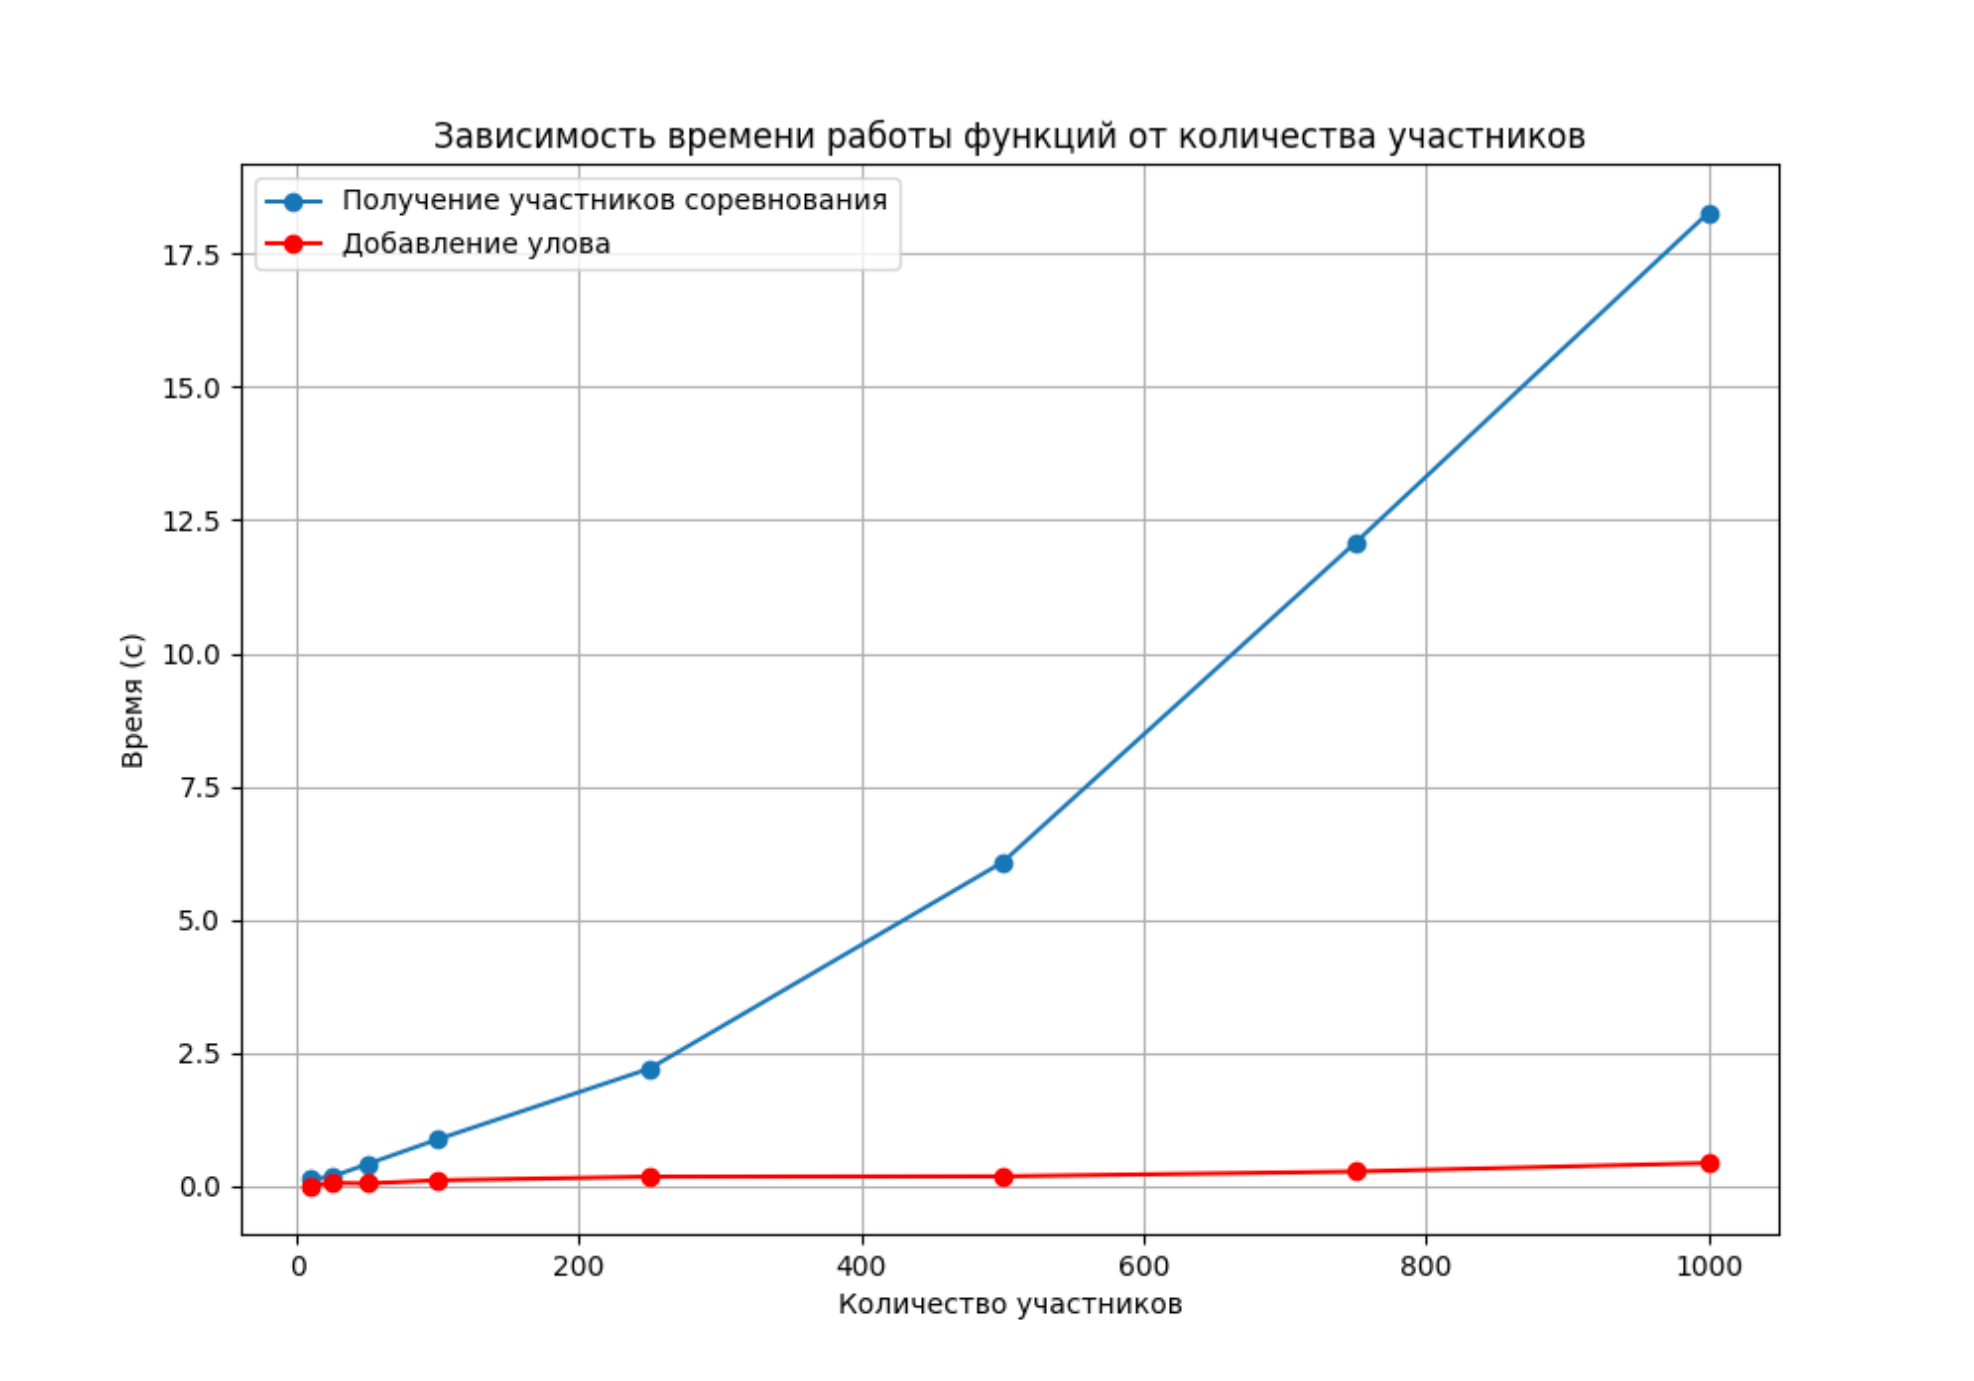
\includegraphics[scale=0.45]{img/plot}}
	\caption{Зависимость времени работы функций от количества участников}
	\label{fig:plot}
\end{figure}

Из результатов измерений можно сделать вывод, что при увеличении количества участников скорость работы функции получения списка участников соревнования изменяется сильнее, чем скорость работы функции добавления улова. Так, при изменении количества участников в 100 раз (от 10 до 1000), время, затрачиваемое на работу функции получения участников, увеличивается в 139 раз, а время, затрачиваемое на работу функции создания улова, увеличивается лишь в 42 раза. 

\subsection{Вывод из раздела}

Исследование показало, что время, затрачиваемое на работу функции получения всех участников соревнования, увеличивается заметно быстрее, чем время, затрачиваемое на работу функции создания улова. Очевидно, что выборка из всей базы --- формирование списка --- будет требовать большее количество времени, чем фиксирование улова, что подтвердило исследование. Это показывает, что при одинаковом количестве спортсменов разные функции могут требовать неодинакового (иногда сильно разнящегося) времени для работы. 
